\begin{abstract}

We introduce a platform for Melanoma Classification, utilizing a technical
infrastructure based on Convolutional Neural Network (CNN) models, specifically
ResNet18.

Exclusively utilizing image data for training and validation, we have refrained
from incorporating additional metadata during the training process. To enhance
model performance, various training strategies such as data augmentation,
learning rate decay, dropout, etc., were employed.

The resulting models are accessible through an API, allowing users to interact
with them via a user-friendly web application. The platform showcases the
effectiveness of CNNs in melanoma classification, underscoring the importance
of easily accessible research.

\end{abstract}


\section{Introduction}

Skin cancer, including melanoma, is a significant global public health concern.
Melanoma presents a considerable challenge due to its high mortality rate and
the critical importance of early detection for successful treatment. Cancer
begins when healthy cells undergo changes that cause them to grow and divide
uncontrollably, forming tumors. These tumors can be classified as either
cancerous (malignant) or non-cancerous (benign) \cite{Melanoma}. \\

In recent times, there has been a growing focus on automating tasks in the
medical field through Computer-Aided Diagnosis (CAD)\footnote{CAD refers to the
use of computer algorithms and technologies to assist healthcare professionals
in the process of medical diagnosis.}. Some studies
\cite{EpidemiologySkinCancer} \cite{SkinCancerDeepLearning} \cite{SkinCancerDeepNN} have demonstrated that
these systems can achieve results similar to those of professionals. However,
the integration of CAD into the medical system remains a significant challenge.
\\

The development of a CAD system necessitates the creation of models capable of
effectively classifying melanoma. The SIIM-ISIC Melanoma Classification
challenge specifically tasks participants with building models for identifying
melanoma using skin lesion images and associated metadata. This thesis outlines
our approach, wherein we leverage data from this challenge to train our models
and subsequently expose them through our platform. By doing so, we contribute
to the ongoing efforts to bridge the gap between cutting-edge medical imaging
technology and practical clinical applications.

\newpage

\section{Objectives}

The final objective of this thesis is to craft a CAD infrastructure, focused on
melanoma detection using deep learning vision models capable of detecting
melanoma on dermoscopy images. To this end, the gradual achievements that must
be accomplished are:

\begin{itemize}

  \item Gaining a comprehensive understanding of the theory behind deep
    learning vision models and its practical applications.

   \item Select a base transfer model. Is the model good enough?, the selection
     of this model is given by the technical limitations or by any other
     justification.

  \item Study different approaches to train the models and select a good
    evaluate metric given the dataset distribution of dermoscopy images.

  \item  Develop the CAD infrastructure. It should contain the  trained models,
    a simple web UI\footnote{User Interface. Is the point of human-computer
    interaction and communication in a device.}, an API\footnote{Application
      Programming Interface. Is a set of protocols, routines, tools, and
    definitions that allow different software applications to communicate with
  each others.} and finally a mechanism using Docker\footnote{Docker is a tool
  for packaging and deploying applications in lightweight, consistent
containers.} to create the images of these services making it ease to deploy in
any system that supports virtualization.

\end{itemize}


\section{Development process}

The project methodology employed in this endeavor follows a continuous process.
The project incorporates the concept of utilizing idle time effectively. For
instance, during the training of models, there are periods of idle time, which
we exploited by concurrently working on other tasks related to developing the
entire infrastructure. This approach allows for maximizing productivity
throughout the project, see Figure \ref{fig:flux_development}.

\newpage

\begin{landscape}

  \begin{figure}[H]
  \centering
  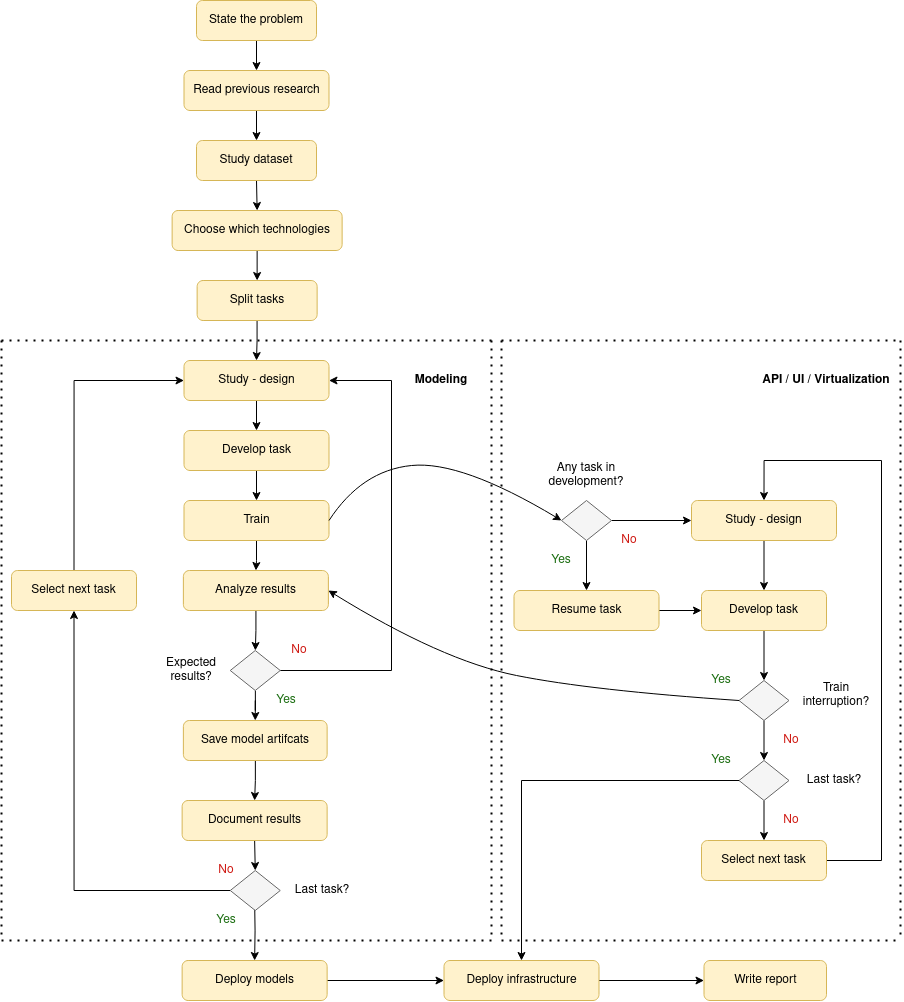
\includegraphics[width=0.82\textwidth]{imatges/planing_and_methodology/EmplyedMethodology.png}
  \caption{\textit{Development process methodology.}}
  \label{fig:flux_development}
  \end{figure}

\end{landscape}

\newpage

\section{CAD infrastructure pipeline}

Our CAD infrastructure pipeline  (see Figure \ref{fig:cad-pipeline}), consists
of different steps, beginning with data acquisition, followed by data
preprocessing. We then set up different datasets for training, validation, and
testing. Subsequently, we train the models and, assess the models gathering
metrics and finally we deploy the models under a crafted API.

\begin{figure}[H]
  %\begin{adjustbox}{width=\textwidth, trim={0.2cm 0pt 1.5cm 0pt}, clip}
  \centering
  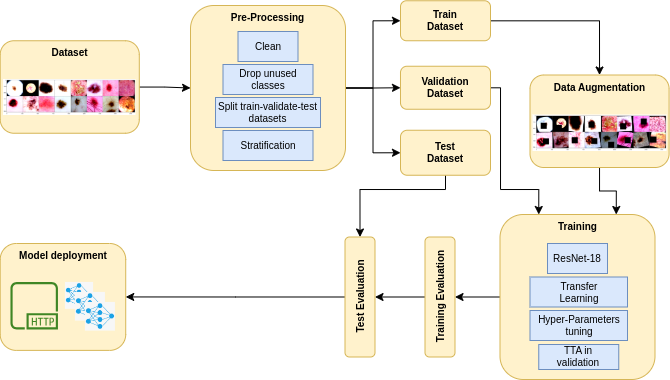
\includegraphics[width=0.9\textwidth]{imatges/methodological_contribution/Pipeline.drawio.png}
  %\end{adjustbox}
  \caption{\textit{CAD infrastructure pipeline. Train, test and deploy. }}
  {\label{fig:cad-pipeline}}
\end{figure}

\section{Data and training strategies}

Inspired by the approach of the Winning Solution to the SIIM-ISIC Melanoma
Classification Challenge \cite{WinningISIC}. The Winning Solution team observed
that in the entire dataset of 2020, comprising 33K images, only 1.76\% were
positive samples (i.e., malignant). In response, they decided to augment this
data by incorporating information from the datasets of the same competition
from the previous years (2018 and 2019). Although the individual datasets from
these earlier years were smaller, totaling 25K images, they exhibited a
positive ratio of 17.85\%. This strategic combination allowed for a more
balanced representation of positive cases in the training data. \\

To build the original dataset, we utilized eight classes selected from the raw
dataset, as the remaining classes we considered not significant or there were
very few samples of them. Any sample that was not categorized as one of the
following classes were excluded from the training process.

\begin{itemize}
  \item melanoma
  \item nevus
  \item BCC (Basal Cell Carcinoma)
  \item BKL (Benign lesions of the keratosis)
  \item AK (Actinic Keratosis)
  \item SCC (Squamous Cell Carcinoma)
  \item VASC (Vascular Lesions)
  \item DF (Dermatofibroma)
\end{itemize}

The filtered dataset comprises 31,265 distinct image samples, demonstrating a
highly imbalanced dataset, as evident from Figure
\ref{fig:hole-dataset-distribution}.

\begin{figure}[H]
  \centering
  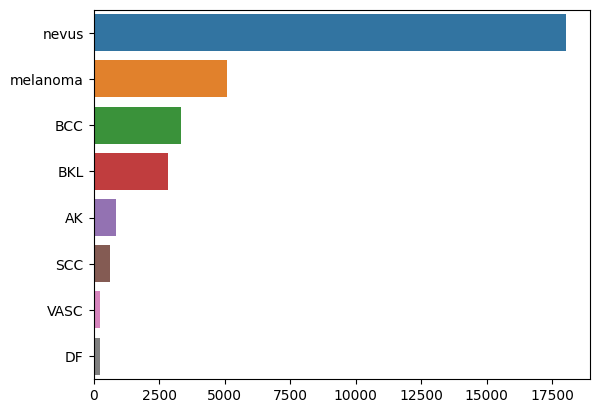
\includegraphics[width=0.75\textwidth]{imatges/data-training-strategies/hole-dataset-diagnosis.png}
  \caption[Categories distribution in dataset]{\textit{Categories distribution in dataset.}}
  {\label{fig:hole-dataset-distribution}}
\end{figure}


We started dividing the original dataset into three subsets using the Holdout
set scheme, see Figure \ref{fig:holdout-test-scheme}. \\

During the training phase, the test set remains completely separate and is not
used in any way to configure the hyper-parameters. This ensures that the
performance of a model on the test set is not artificially inflated by
adjusting hyper-parameters to achieve an exceptionally good outcome in the validation set. \\

\newpage

The data from the ISIC Archive was divided using the following percentages: 80\%
for training, 10\% for validation, and 10\% for testing. Each subset contain the same
distribution of classes as the original dataset, i.e., we applied stratification.

\begin{figure}[H]
  \centering
  \begin{adjustbox}{width=0.7\textwidth, trim={0cm 1cm 0cm 1.25cm}, clip}
    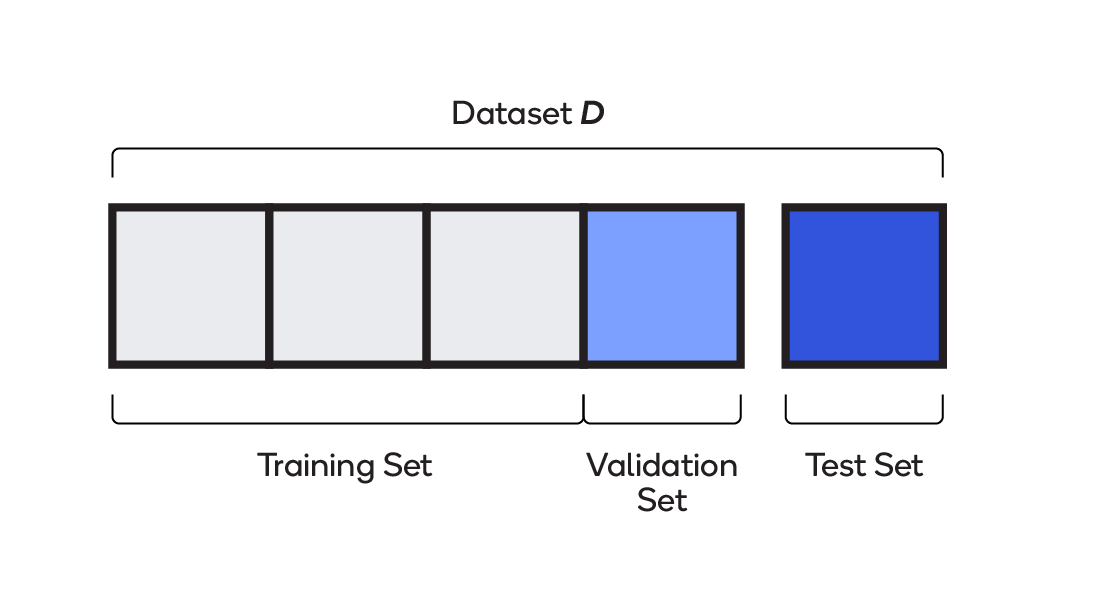
\includegraphics[width=\textwidth]{imatges/data-training-strategies/train-test-validation-sets.png}
  \end{adjustbox}
  \caption[Holdout set scheme]{\textit{Holdout set scheme. Illustration by Qualcomm}}
  {\label{fig:holdout-test-scheme}}
\end{figure}

In small to medium sized datasets, augmentation is important to prevent
overfit. For some of our trained models, we used in the training dataset our
augmentation pipelines, as illustrated in Figure \ref{fig:sample-of-datasets} and
Figure \ref{fig:aug-sample-of-datasets}, with contains the following augmentations
from the popular and powerful PyTorch augmentation library Albumentations
\cite{Albumentations}: Transpose, Flip, Rotate, RandomBrightness,
RandomContrast, MotionBlur, MedianBlur, Gaus- sianBlur, GaussNoise,
OpticalDistortion, GridDistortion, ElasticTransform, CLAHE, HueSaturationValue,
ShiftScaleRotate, Cutout.

\begin{figure}[H] \centering
  \begin{adjustbox}{width=0.9\textwidth}
    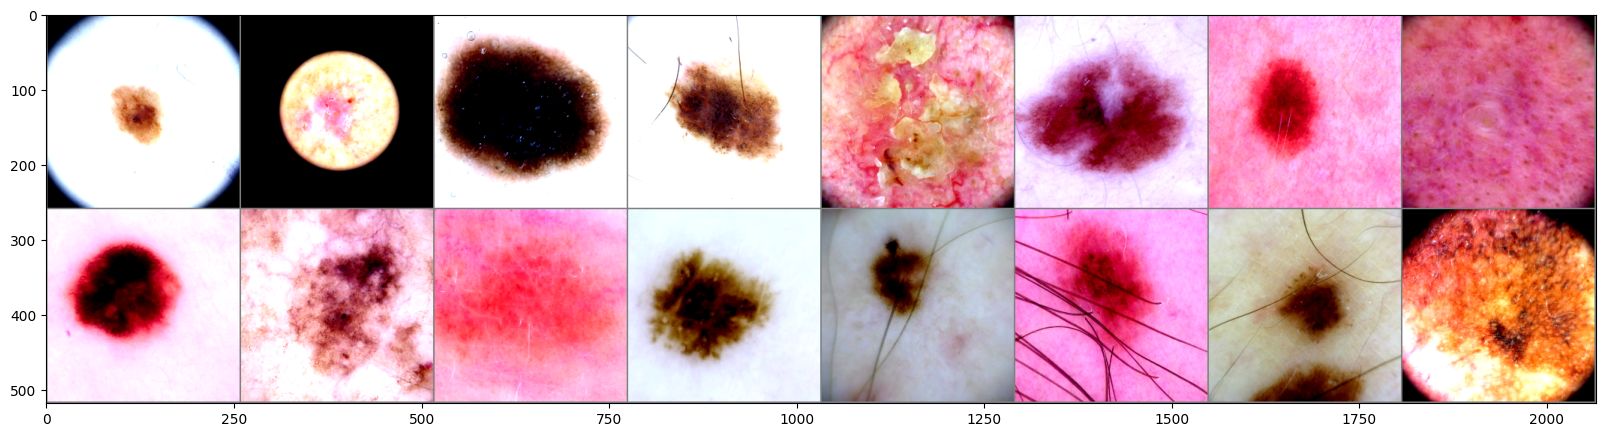
\includegraphics[width=\textwidth]{imatges/methodological_contribution/random-sample-of-isic.png}
  \end{adjustbox}
  \caption[Random sample of images]{\textit{Random sample of images.}}
  {\label{fig:sample-of-datasets}}
\end{figure}

\begin{figure}[H]
  \centering
  \begin{adjustbox}{width=0.9\textwidth}
  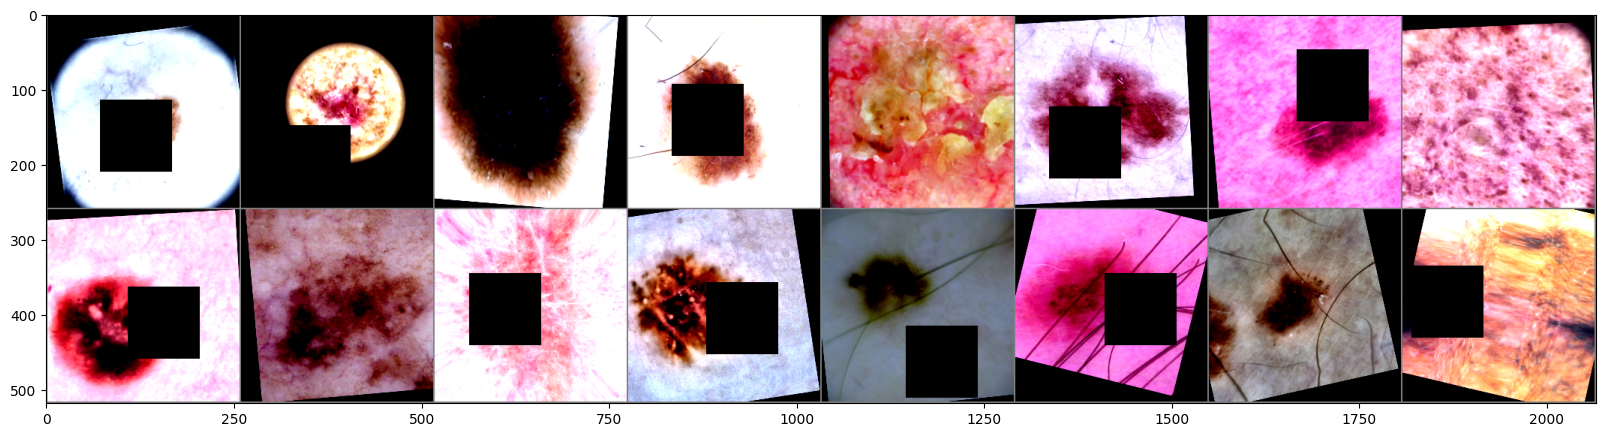
\includegraphics[width=\textwidth]{imatges/methodological_contribution/random-sample-of-isic-augmented.png}
  \end{adjustbox}
  \caption[Augmented random sample of images]{\textit{Augmented random sample of images.}}
  {\label{fig:aug-sample-of-datasets}}
\end{figure}


We decided to use as transfer model an already trained ResNet in the ImageNet
database. ResNet is short for "Residual Network," is a deep convolutional
neural network (CNN) architecture that was introduced in 2015 by researchers
from Microsoft Research \cite{ResNetPaper}. It revolutionized the field of deep
learning by addressing the challenge of training very deep neural networks. \\

There are various architectural variants or "flavors" of ResNet, including
ResNet-152,  ResNet-101,  ResNet-50,  ResNet-34, and  ResNet-18. The number
following the name of each ResNet variant indicates the number of inner layers
present in the architecture. The more the number of the layers the more the
accuracy, yet the number of parameters to be trained increase. To accurately
assess the performance of each ResNet architecture refer to Table
\ref{table:resnet}.

\begin{table}[H]
  \centering
  \begin{tabular}{lcc}
    \toprule
    \textbf{Model} & \textbf{Accuracy} & \textbf{Parameters} \\
    \midrule
    ResNet-152 & 78.31\% & 60.2M \\
    ResNet-101 & 77.37\% & 44.5M \\
    ResNet-50 & 76.15\% & 25.6M \\
    ResNet-34 & 73.30\% & 21.8M \\
    ResNet-18 & 69.76\% & 11.7M \\
    \bottomrule
  \end{tabular}
  \caption[Accuracy achieved on ImageNet and trainable parameters of each ResNet]
  {\textit{Accuracy achieved on ImageNet and trainable parameters of each ResNet.
  Each image in the ImageNet dataset is associated with 1 of 1,000 classes. Table by paperswithcode}}
  {\label{table:resnet}}
\end{table}

We decided to use ResNet18 as base model only for technical reasons and time
constrains. The lack of powerfull GPUs took us to pick this estimator and not
other. There are other lightweight architectures that we could have tried as:
AlexNet, ResNetXt, VGG, etc, but finding the model that performance the best in
the SIIM-ISIC Melanoma competition is not the goal of this thesis. \\

Upon the ResNet18 we propose two models. For both models, we transformed the
ResNet18's last layer into an identity layer, i.e., \(\mathbf{y} =
Identity(\mathbf{y}), \quad \mathbf{y} \in \mathbb{R}^{512}\) and added a new
trainable linear layer, \(\mathbf{y} = Linear(\mathbf{x}), \quad \mathbf{y} \in
\mathbb{R}^8, \quad \mathbf{x} \in \mathbb{R}^{512}\). \\

To train the models, we only need to define the forward propagation. The result
of the forward propagation for the first model is given by:

\[ \mathbf{y} = Forward(\mathbf{x}) = Linear(ResNet18(\mathbf{x})), \]

where \( \mathbf{y} \in \mathbb{R}^8 \), and \( \mathbf{x}  \in
\mathbb{R}^{3 \times 256 \times 256} \). Figure \ref{fig:resnet-18-melanoma-arch} shows
the architecture of the first model.

\begin{figure}[H]
  \centering
  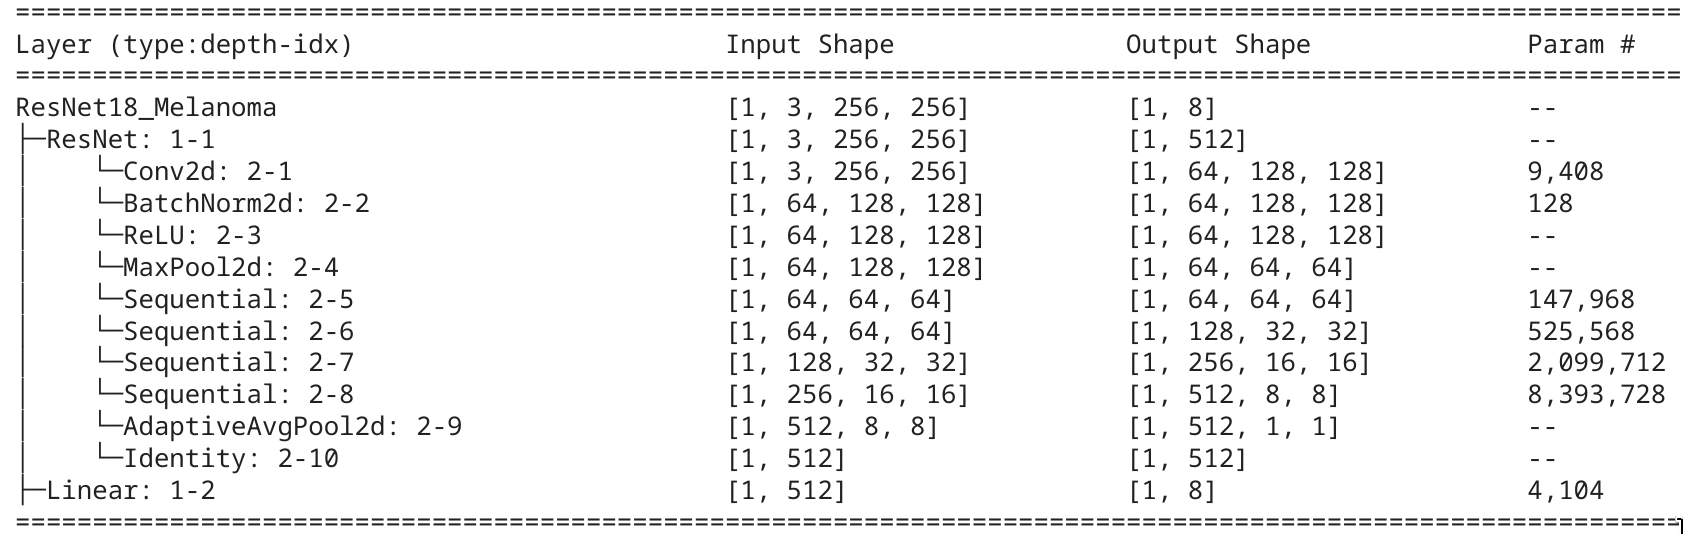
\includegraphics[width=\textwidth]{imatges/methodological_contribution/ResNet18_Melanoma.png}
  \caption[ResNet18\_Melanoma architecture]{\textit{ResNet18 Melanoma architecture.}}
  {\label{fig:resnet-18-melanoma-arch}}
\end{figure}

The forward propagation of the second model is more intricate, involving the
averaging of predictions \(N\) times through the application of the function
composition \(Linear \circ Dropout\). Dropout is a stochastic regularization
technique \cite{DropoutPaper}.

\[ \quad \mathbf{y} = Forward(\mathbf{x}) = \frac{\sum_{j=1}^{N} Linear(Dropout(\mathbf{r}))}{\mathbf{N}}, \]

where \( \mathbf{y} \in  \mathbb{R}^8 \), \( \mathbf{x}  \in \mathbb{R}^{3
\times 256 \times 256} \),  and \(\mathbf{r} = ResNet18(\mathbf{x}), \quad
\mathbf{r} \in \mathbb{R}^{512}\). Figure
\ref{fig:resnet-18-dropout-melanoma-arch} shows the architecture of the second
model.

\begin{figure}[H]
  \centering
  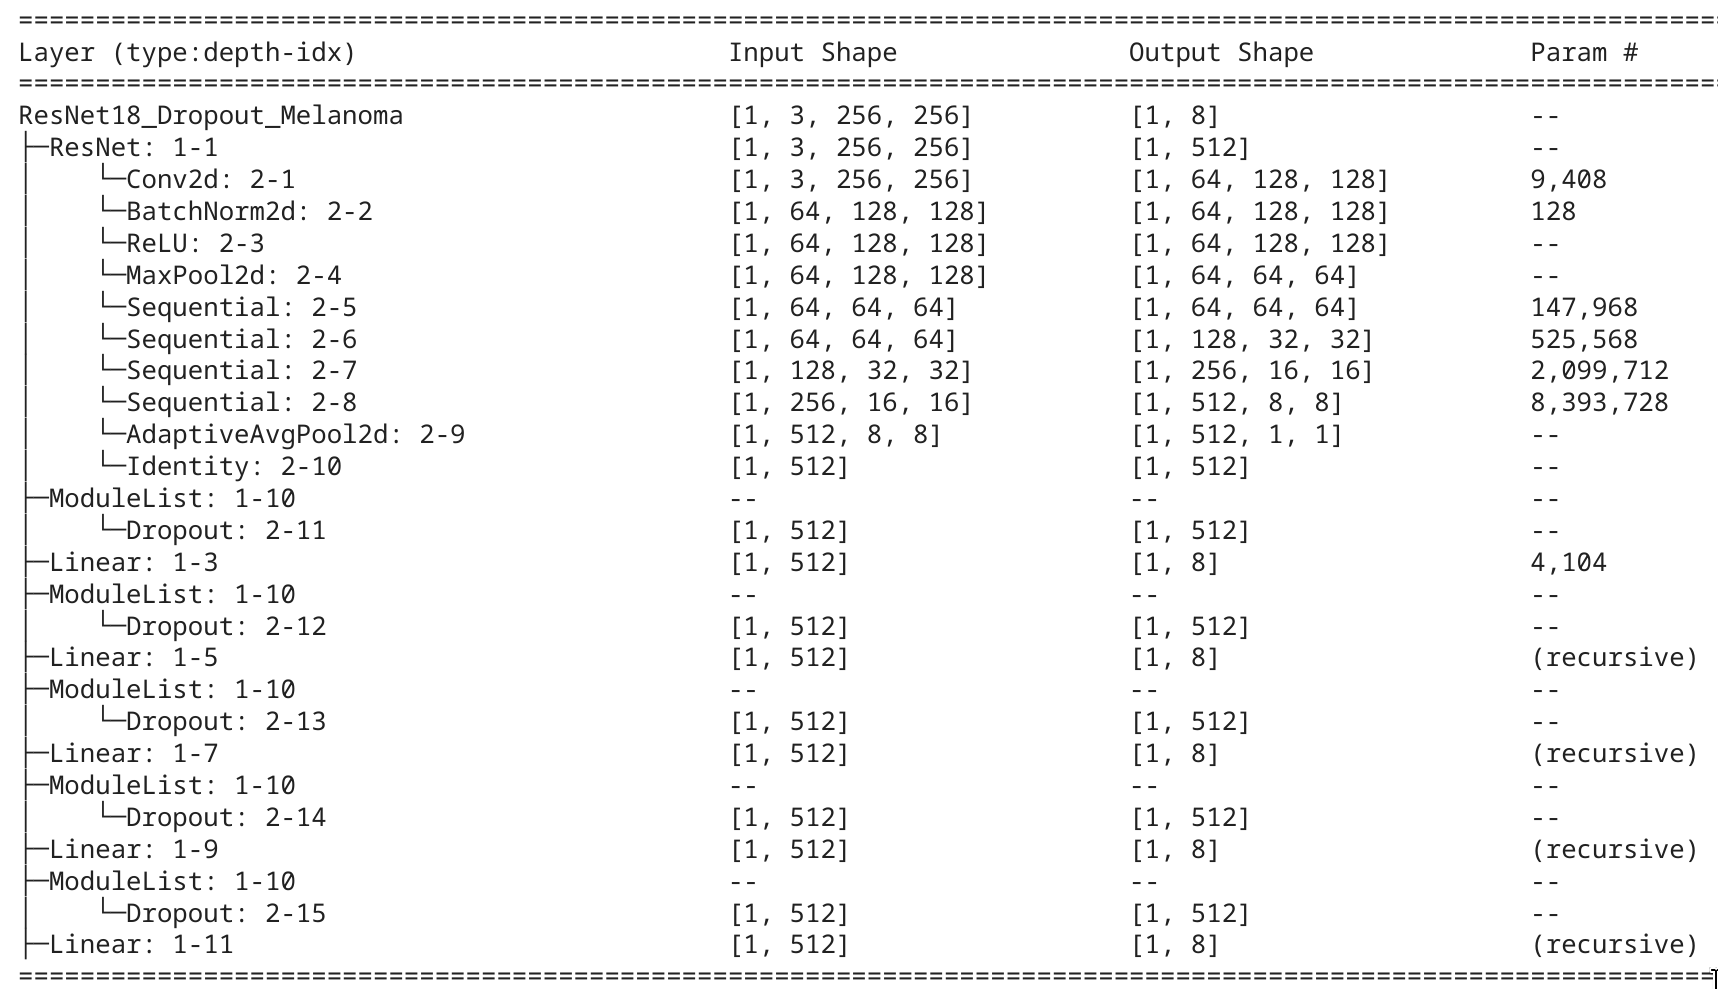
\includegraphics[width=\textwidth]{imatges/methodological_contribution/ResNet18_Dropout_Melanoma.png}
  \caption[ResNet18\_Dropout\_Melanoma architecture]{\textit{ResNet18 Dropout Melanoma architecture.}}
  {\label{fig:resnet-18-dropout-melanoma-arch}}
\end{figure}


\section{Validation strategy}

In any machine learning project, it is critical to establish a reliable
validation scheme to properly evaluate and compare models. This becomes
particularly crucial when dealing with a small to medium-sized dataset or when
the evaluation metric is unstable, as is the case with the dataset provided in
the competition. There are various metrics commonly used to assess the quality of a model's
predictions. We present a selection of metrics that we find relevant for
evaluating our models. \\

A confusion matrix (see Figure \ref{fig:confusion-matrix}) is a square matrix
with dimensions \(N\times N\) where \(N\) represents the total number of classes being
predicted.

\begin{figure}[H]
  \begin{adjustbox}{trim={0pt 0.5cm 0pt 1cm}, clip}
    \centering
    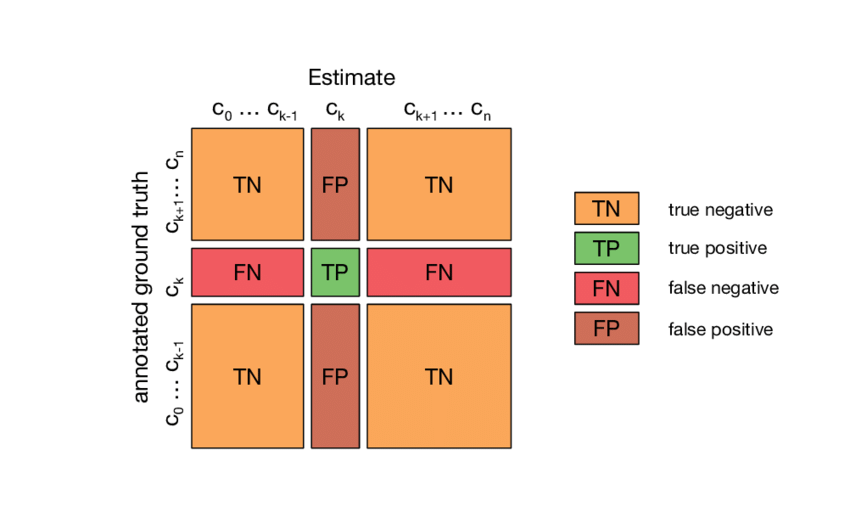
\includegraphics[width=0.9\textwidth]{imatges/validation-strategy/confusion-matrix.png}
  \end{adjustbox}
  \caption[Confusion matrix multi-class]{\textit{Confusion matrix multi-class. Illustration by kaggle}}
  {\label{fig:confusion-matrix}}
\end{figure}

From confusion matrix we can obtain other metrics such as:

\begin{itemize}

  \item {\bf Accuracy}

    The Accuracy metric, calculates the ratio of correct predictions to the total number of
    predictions made on a dataset. It is not a good matric when working with
    unbalanced datasets.

    \[Accuracy = \frac{TP + TN}{TP + TN + FP + FN}\]

  \item {\bf True Positive Rate (TPR) or Sensitivity}

    The True Positive Rate tells about how many of the true class samples were
    correctly classified.

    \[TPR = \frac{TP}{TP + FN}\]


  \item {\bf False Positive Rate (FPR) or False Alarm Ratio}

    The False Positive Rate tells the proportion of the true class samples that
    were not correctly classified and are False Positive.

    \[FPR = \frac{FP}{FP + TN}\]


  \item {\bf Receiver Operator Characteristic (ROC)}

  An ROC curve plots TPR vs. FPR at different classification thresholds \(T\),
  where $0 <= T <= 1$. Lowering the classification threshold
  classifies more items as positive, thus increasing both False Positives and
  True Positives. By plotting the curve, you can say which threshold is better,
  depeding on how many False Positives we are willing to accept.

    \begin{figure}[H]
      \centering
      \begin{adjustbox}{trim={0pt 0cm 0pt 0cm}, clip}
        \centering
        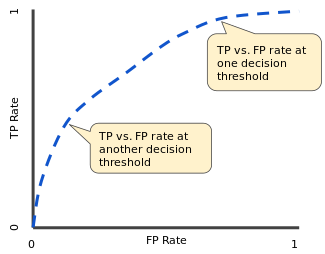
\includegraphics[width=0.55\textwidth]{imatges/validation-strategy/ROCCurve.png}
      \end{adjustbox}
        \caption{\textit{Typical ROC Curve. Illustration by Alphabet Inc.}}
      {\label{fig:ROCCurve}}
    \end{figure}


  \item {\bf Area Under the Curve (AUC)}

  Area Under the Curve is a value between 0 and 1 that measures the
  ability of a classifier to distinguish between classes. It is used as a summary of
  the ROC curve. The higher the AUC, the better the performance of the model at
  distinguishing between the positive and negative classes.

  \begin{figure}[H]
    \centering
    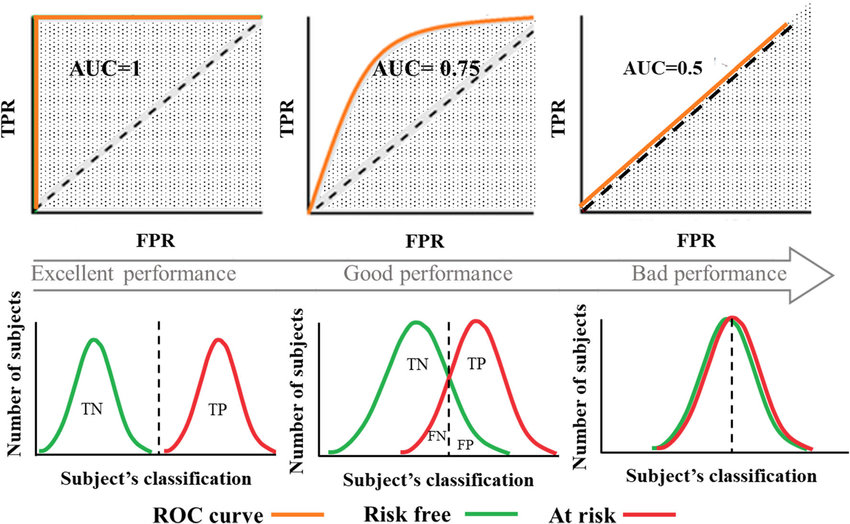
\includegraphics[width=0.7\textwidth]{imatges/validation-strategy/auc.png}
    \caption[AUC-ROC performance]{\textit{AUC comparation. Illustration by Elizabeth Louise Thomas}}
    {\label{fig:auc-roc}}
  \end{figure}

\end{itemize}

We used Test-time augmentation (TTA) \cite{TTA} in the inference phases, i.e., validation
and testing. The idea behind TTA, is to generate multiple augmented versions of
the test input and average the predictions of the model over these augmented
samples to get a more robust and accurate result. \\

Let's denote the original test input as \(X\) and the model's prediction for
\(X\) as \(Y\). TTA involves generating \(N\) augmented versions per each
\(X_i\), obtaining predictions for each of these augmented samples (\(Y_i^1, Y_i^2,
..., Y_i^N\)), and then averaging these predictions.

\[ TTA(X_i) = \frac{1}{N} \sum_{j=1}^{N} f(j, Y_i^j) \]

Where:

\begin{itemize}
  \item \(X\) is the original test input.
  \item \(Y\) is the model's prediction for the original input.
  \item \(X_i\) represents the \(i\)-th augmented version of the test input.
  \item \(Y_i\) is the model's prediction for the \(i\)-th augmented input.
  \item \(N\) is the number of augmented samples generated.
  \item \(f\) is defined as \(f: Int \rightarrow X \rightarrow X\). The
    function applies simple transformations such as rotations and flips.
\end{itemize}


\section{Model metrics}

The training phase ended with the development of eight models. Various learning
policies such as; Learning Decay with schedulers and regularization with Data
Agumentation and Dropout were applied. We computed other metrics such as,
recall and presition but in Table \ref{table:resume-metrics} we show the AUC
metric of in all datasets for all models. \\

The metrics with a gray background in Table \ref{table:resume-metrics}
are from models that incorporated additional regularization techniques. These
models were trained for 40 epochs since regularization tends to slow down the
minimization of the objective function compared to the other models that were
trained for only 20 epochs. \\

Models that used a scheduler during the training stage are denoted with a
symbol next to their names. For reference, the mapping between the scheduler
used and the corresponding symbol is provided in Table
\ref{table:scheduler-mapping}.

\begin{table}[H]
  \centering
  \begin{tabular}{cc}
    \toprule
    \multicolumn{2}{c}{\textbf{Scheduler Mapping}} \\
    \midrule
    $\star$     & Step Learning Rate \\
    $\ast$      & Cosine Annealing Learning Rate \\
    $\bullet$   & Cosine Annealing Warm Restarts \\
    \bottomrule
  \end{tabular}
  \caption[Scheduler mapping]
  {\textit{Scheduler mapping.}}
  \label{table:scheduler-mapping}
\end{table}


\begin{table}[H]
    \centering
    \begin{tabular}{lrrr}
      \toprule
      & \textbf{Train AUC} & \textbf{Val AUC} & \textbf{Test AUC} \\
      \midrule
      M0 & 0.952 & 0.903 & 0.892  \\
      M1 $\star$ & 0.947 & 0.900 & 0.892 \\
      M2 $\ast$ & 0.933 & 0.895 & 0.885 \\
      M3 $\bullet$ & 0.935 & 0.896 & 0.886 \\
      \midrule
      \cellcolor{gray!50}M4 & \cellcolor{gray!50}0.886 & \cellcolor{gray!50}0.877 & \cellcolor{gray!50}0.858 \\
      \cellcolor{gray!50}M5 $\star$ & \cellcolor{gray!50}0.867 & \cellcolor{gray!50}0.861 & \cellcolor{gray!50}0.843 \\
      \cellcolor{gray!50}M6 $\ast$ & \cellcolor{gray!50}0.874 & \cellcolor{gray!50}0.868 & \cellcolor{gray!50}0.848 \\
      \cellcolor{gray!50}M7 $\bullet$ & \cellcolor{gray!50}0.877 & \cellcolor{gray!50}0.869 & \cellcolor{gray!50}0.849 \\

      \midrule

      Mean &  94.175\% & 89.850\% & 88.875\%  \\
      SD   & 0.921\% & 0.370\% & 0.377\%  \\

      \midrule

      \cellcolor{gray!50}Mean & \cellcolor{gray!50}87.600\% & \cellcolor{gray!50}86.875\% & \cellcolor{gray!50}84.950\% \\
      \cellcolor{gray!50}SD & \cellcolor{gray!50}0.787\% & \cellcolor{gray!50}0.655\% & \cellcolor{gray!50}0.625\% \\

      \bottomrule
    \end{tabular}
    \caption[Metrics in the datasets]
    {\textit{AUC metric in all datasets. }}
    {\label{table:resume-metrics}}
  \end{table}


As a result, we conclude that the first group of models performed well on the
test set with an average AUC of 88.875\% and a small standard deviation of
±0.377\%. However, they showed signs of overfitting in the training process, as
model performed excelent in the training data but poorer in the validation set.
In contrast, the second group of models that were trained with additional
regularization techniques, achieved lower results in the test set, but did not
suffer from overfitting. They had an average AUC of 84.950\% with a standard
deviation of ±0.625\%.

\section{CAD infrastructure result}

In this section, we briefly present the CAD infrastructure in its entirety (see
Figure \ref{fig:background-task}). The CAD infrastructure essentially consists
of two services: an API used to expose and interact with the trained models via
the HTTP protocol, and a web application (UI). The UI features a simple layout
that displays prediction data and metadata for dermoscopy images, along with
information about the model used for the prediction. For each service, we
created a Docker image to facilitate easy deployment of the infrastructure on
any system that supports virtualization. \\

The necessary steps to install the infrastructure are explained in the README
of the repository where the research and source code are available. Please
visit the repository at
\href{https://github.com/wilberquito/melanoma.thesis}{https://github.com/wilberquito/melanoma.thesis}.


\begin{figure}[H]
  \centering
  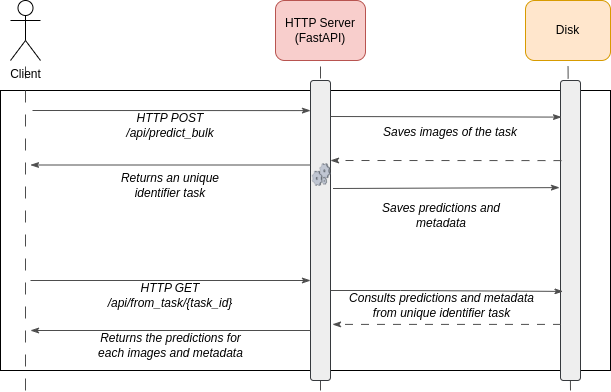
\includegraphics[width=0.9\textwidth]{imatges/cad-result/BackgroundTask.drawio.png}
  \caption{Comunication protocol for infering a bulk of dermoscopy images.}
  {\label{fig:background-task}}
\end{figure}

The API basically has 5 end-points.

\begin{itemize}
  \item {\bf Consult the exposed models}


Request:

\begin{Verbatim}[fontsize=\scriptsize]
http://<api>/public_models
\end{Verbatim}

Possible response:

\begin{Verbatim}[fontsize=\scriptsize]
{
  "models": [
    "M0",
    "M1",
    "M2",
    "M3",
    "M4",
    "M5",
    "M6",
    "M7",
    "vicorobot.8c_b3_768_512_18ep_best_20_fold0",
    "vicorobot.8c_b3_768_512_18ep_best_fold0",
    "vicorobot.8c_b3_768_512_18ep_final_fold0"
  ]
}
\end{Verbatim}



  \item {\bf Trigger inference for a simple image}

This endpoint expects an HTTP request containing a JPEG image in the body,
along with the specified model name for performing the inference.

Request:

\begin{Verbatim}[fontsize=\scriptsize]
POST http://<api>/predict?model_id=<model-id>
\end{Verbatim}

Possible response:

\begin{Verbatim}[fontsize=\scriptsize]
{
  "task_uuid": "721445f5-ff37-4c99-af74-7157925b4a7c"
}
\end{Verbatim}


  \item {\bf Trigger inference for a bulk of images}

This endpoint is designed to handle requests for predicting multiple images
simultaneously. To use this endpoint, you are required to provide two pieces of
information in the HTTP request: the model you wish to use for image inference
and a list of images attached to the request body.

Request:

\begin{Verbatim}[fontsize=\scriptsize]
http://<api>/predict_bulk?model_id=<model-id>
\end{Verbatim}

Possible response:

\begin{Verbatim}[fontsize=\scriptsize]
{
  "task_uuid": "77d5e834-60a1-49b6-a71a-b3472dc21ce5",
  "num_images": 2
}
\end{Verbatim}


  \item {\bf Consult the results of a triggered inference}

Given the unique identifier for a triggered task inference, we can consult the
result of the inference.

Request:

\begin{Verbatim}[fontsize=\scriptsize]
http://<api>/from_task/<task_uuid>
\end{Verbatim}

Possbile response:


\begin{Verbatim}[fontsize=\scriptsize]
[
  {
    "name": "ISIC_0052349.jpg",
    "probabilities": {
      "AK": 0.0007466986,
      "BCC": 0.0005002805,
      "BKL": 0.015733117,
      "DF": 0.00086343783,
      "SCC": 0.0007902466,
      "VASC": 0.0017217622,
      "melanoma": 0.017426228,
      "nevus": 0.9622182
    },
    "metadata": {
      "origin": "wilberquito",
      "net_type": "resnet18",
      "img_size": 256,
      "out_dim": 8
    },
    "prediction": {
      "target": false,
      "label": 7,
      "prediction": "nevus"
    }
  },
  {
    "name": "ISIC_1766619.jpg",
    "probabilities": {
      "AK": 0.00016253705,
      "BCC": 0.00011373816,
      "BKL": 0.00052201655,
      "DF": 0.0006251502,
      "SCC": 0.00032183932,
      "VASC": 0.00025595966,
      "melanoma": 0.0012655357,
      "nevus": 0.9967333
    },
    "metadata": {
      "origin": "wilberquito",
      "net_type": "resnet18",
      "img_size": 256,
      "out_dim": 8
    },
    "prediction": {
      "target": false,
      "label": 7,
      "prediction": "nevus"
    }
  }
]
\end{Verbatim}



  \item {\bf Consult the public end-points}

All end-points are easy accessible by consulting the documentation.

\begin{Verbatim}[fontsize=\scriptsize]
http://<api>/docs
\end{Verbatim}


\end{itemize}

Inspired by the CNN Explainer \cite{CNNExplainer}, we decided not just to
create an API to interact with the model but to craft a UI service where
professionals can immediately interact with the models. It's worth noting that
the resulting UI is a single-page web application with several interactive
buttons (see Figure \ref{fig:ui-tools}).

\begin{figure}[H]
  \centering
  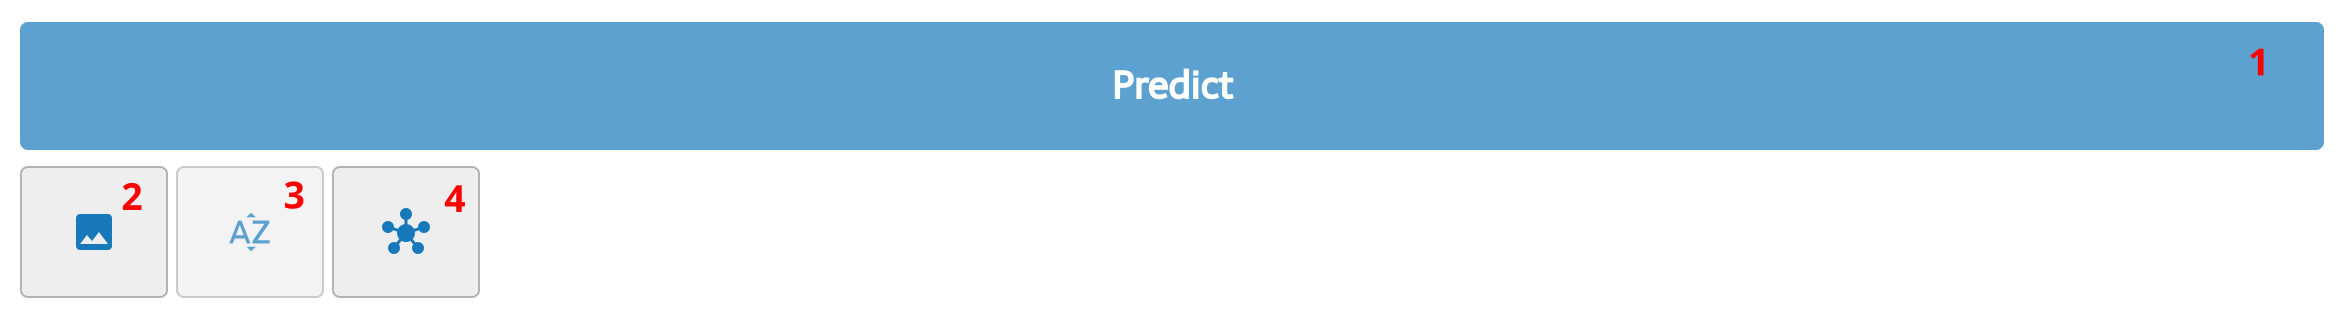
\includegraphics[width=\textwidth]{imatges/results/ui-tools.png}
  \caption[Main interactive buttons of the UI service]{\textit{Main interactive buttons of the UI service. }}
  {\label{fig:ui-tools}}
\end{figure}


\begin{enumerate}

  \item This button serves a dual purpose based on the UI's current state.
    Either allows user make the prediction request or reset the UI clearing the
    results of a inference.

  \item This button enables users to load images directly from their device,
    see Figure \ref{fig:selecting-imgs} and Figure \ref{fig:loaded-images}.

\begin{figure}[H]
  \centering
  \begin{adjustbox}{width=0.8\textwidth, trim={0.05cm 1.25cm 0cm 0.1cm}, clip}
    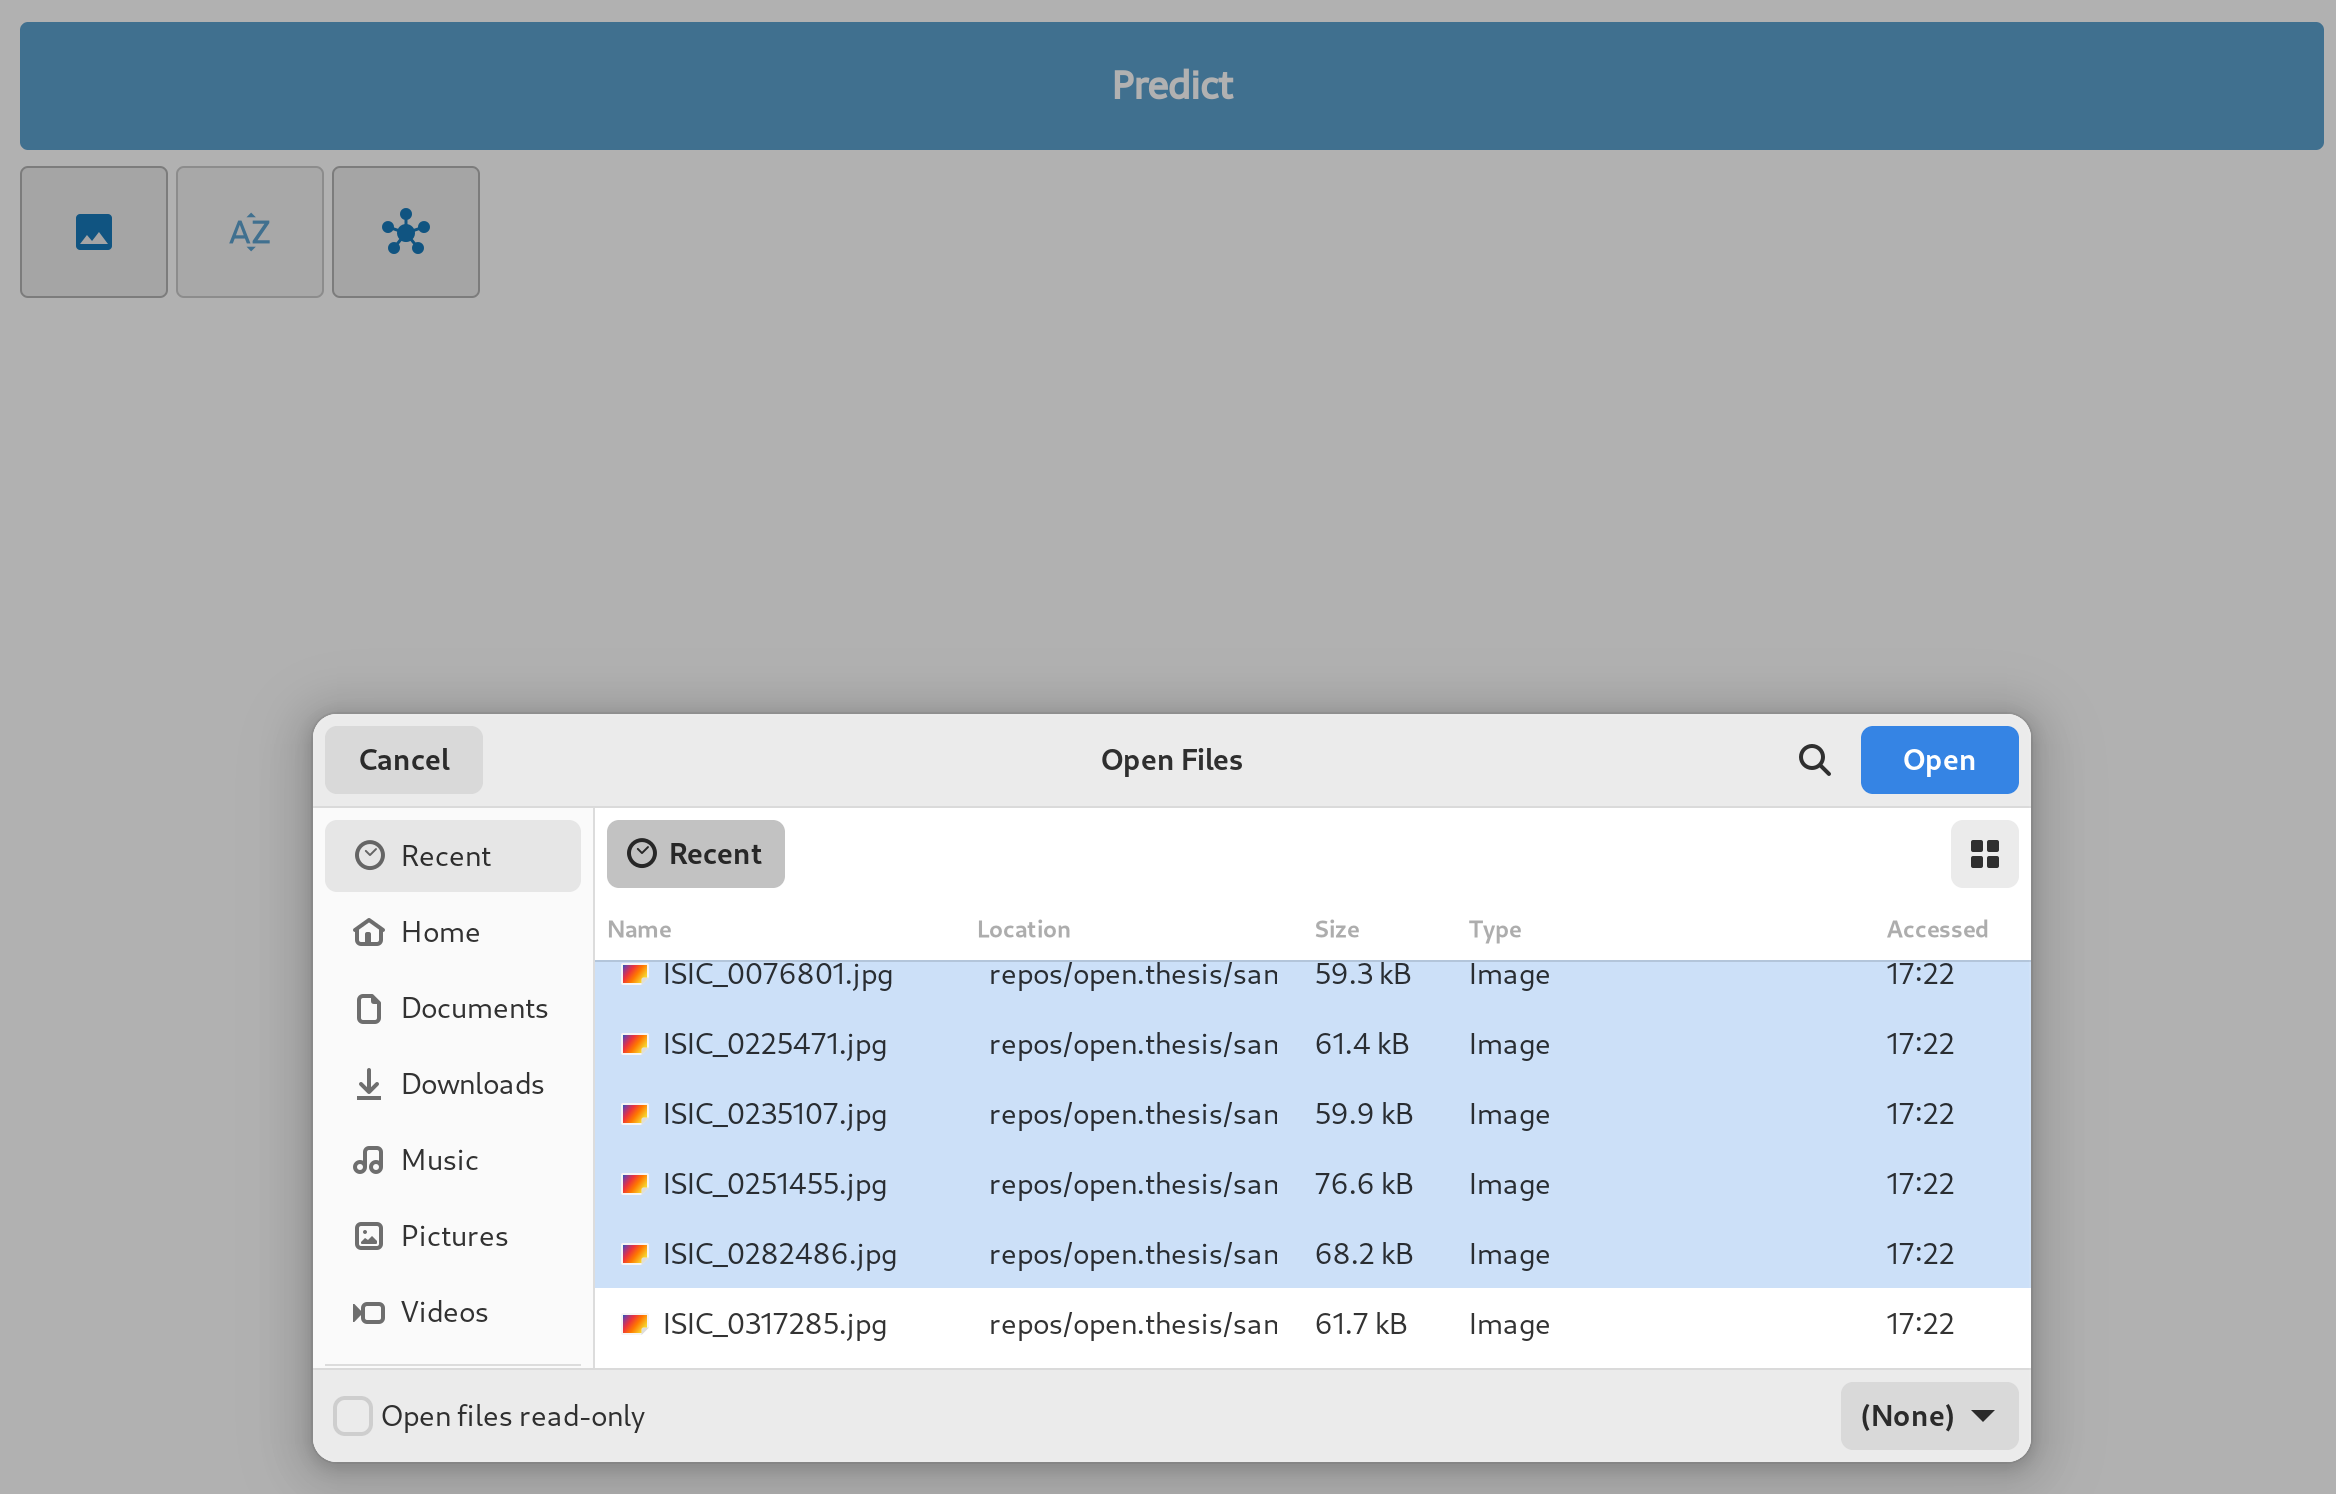
\includegraphics[width=\textwidth]{imatges/results/selecting-images.png}
  \end{adjustbox}
  \caption[Loading dermoscopy images from device]{\textit{Loading dermoscopy images from device.}}
  {\label{fig:selecting-imgs}}
\end{figure}

\begin{figure}[H]
  \centering
  \begin{adjustbox}{width=0.9\textwidth, trim={0cm 3.5cm 0cm 0cm}, clip}
    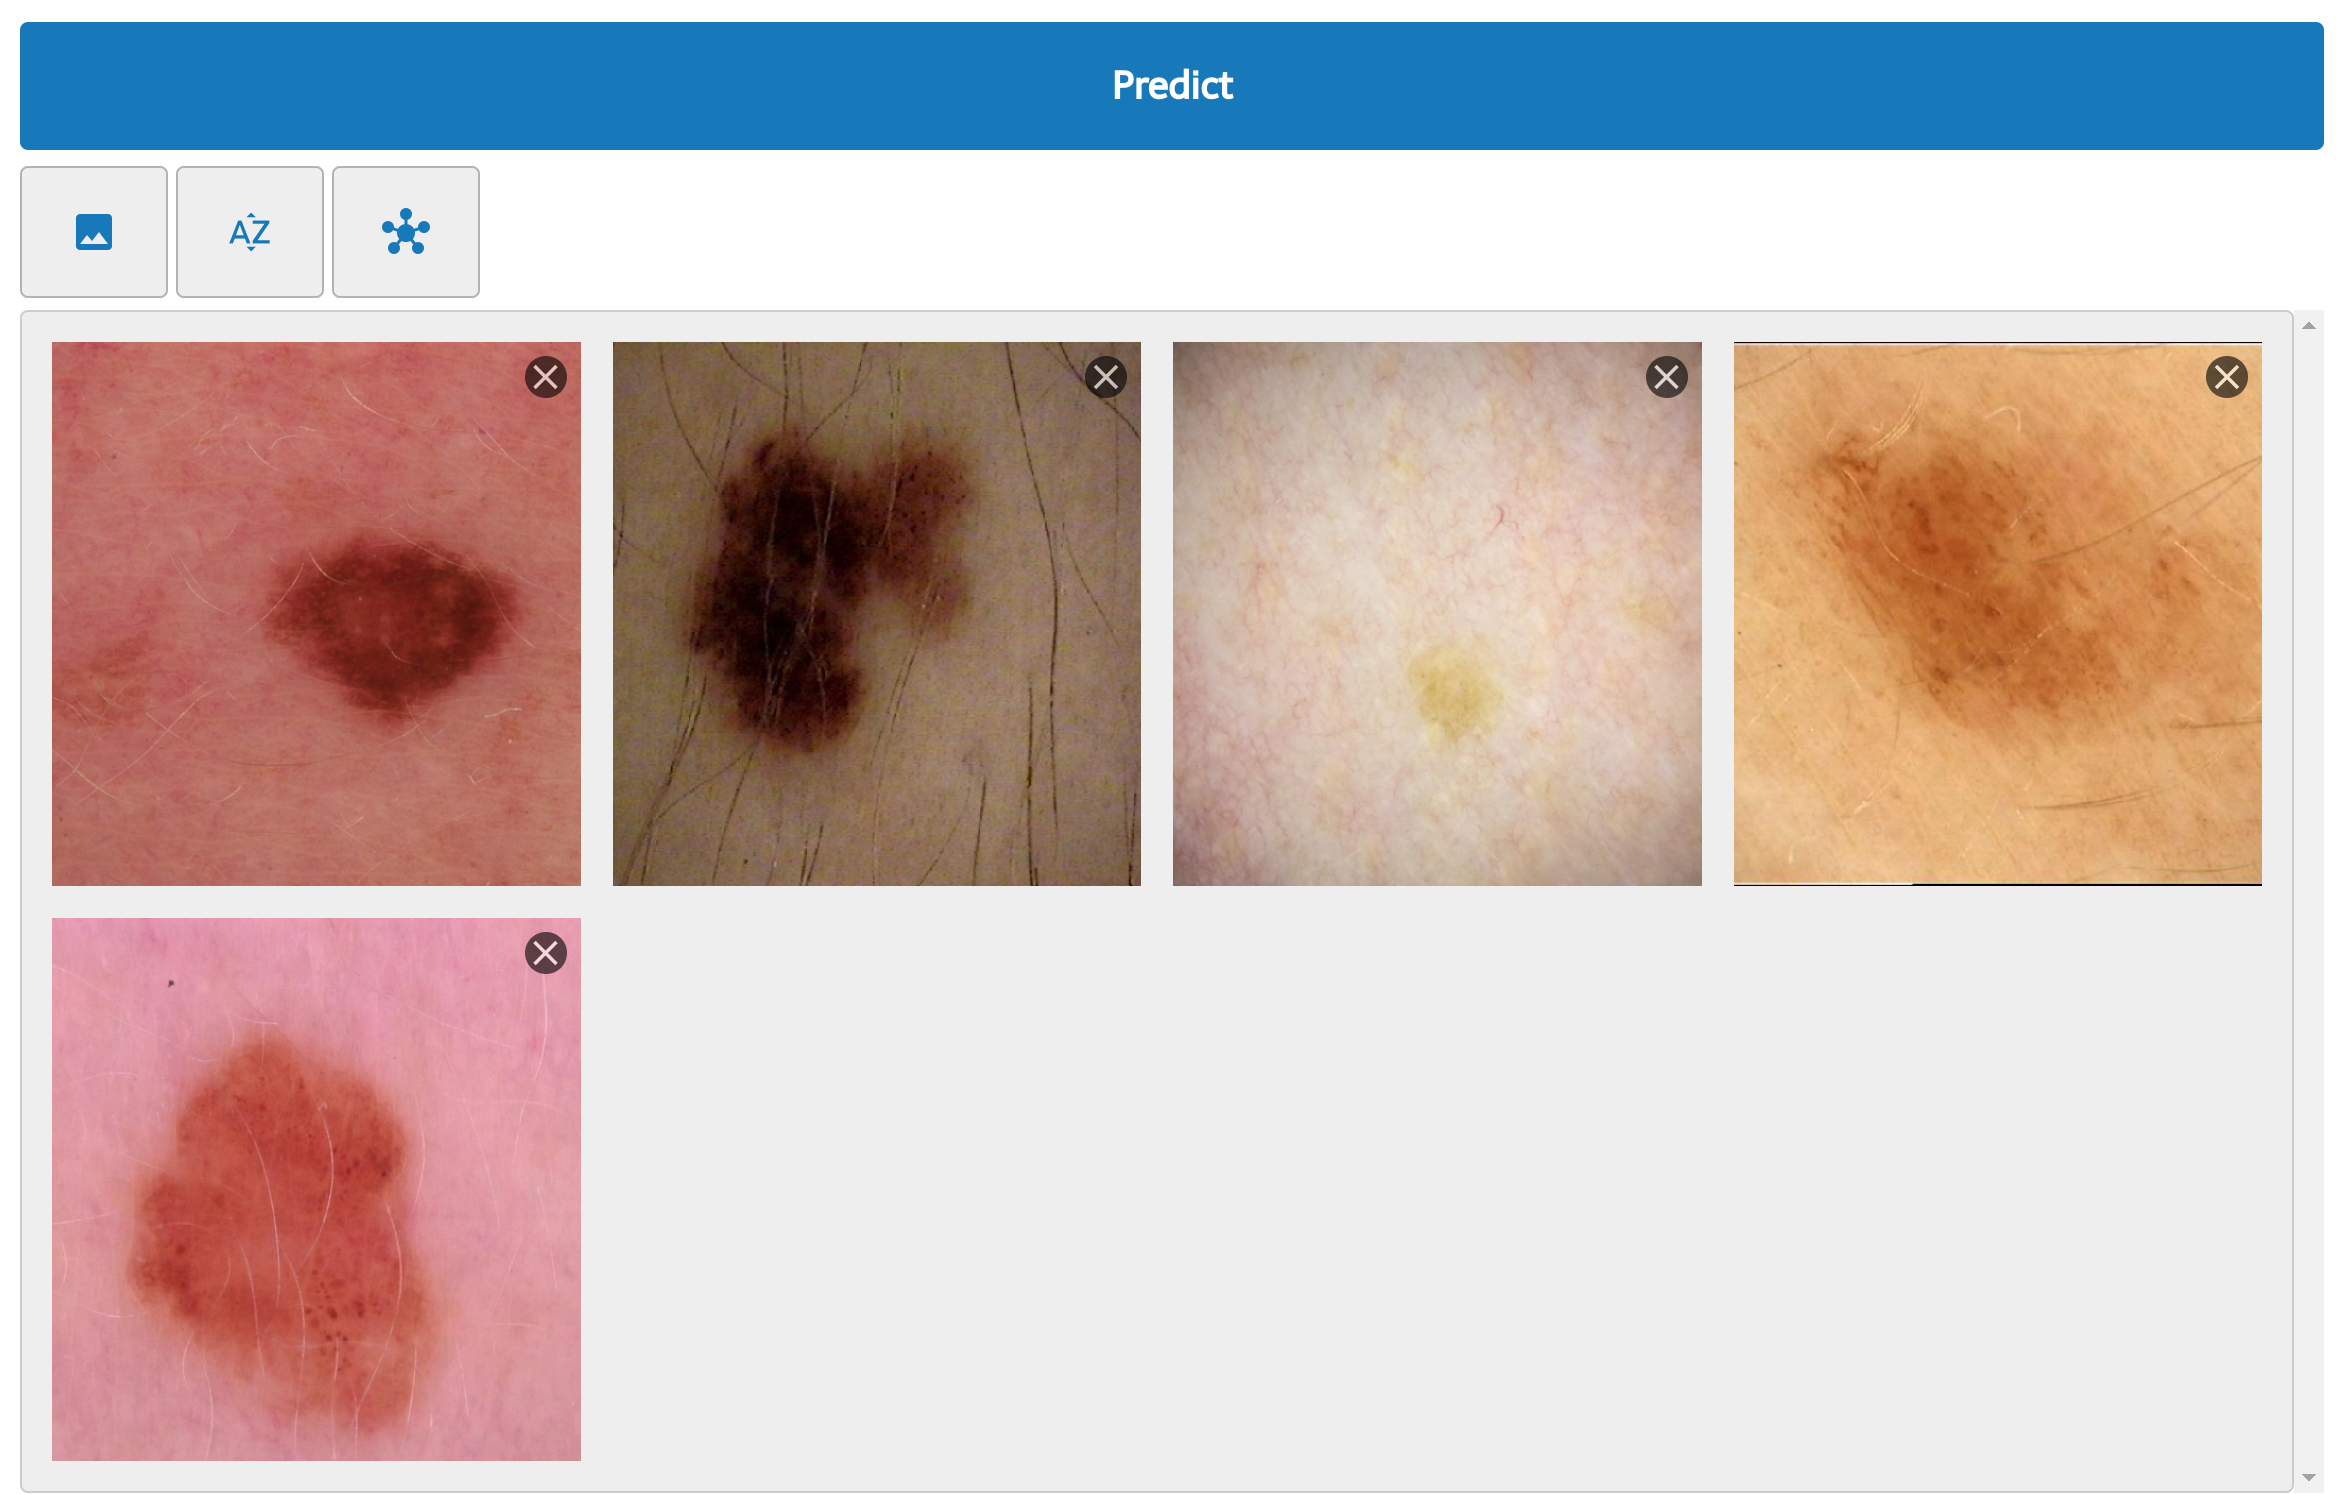
\includegraphics[width=\textwidth]{imatges/results/loaded-images.png}
  \end{adjustbox}
  \caption[Dermoscopy images loaded in the UI]{\textit{Dermoscopy images loaded in the UI. }}
  {\label{fig:loaded-images}}
\end{figure}

  \item Designed to sort the loaded images in the UI, this button operates
    differently depending on whether the inference has been performed. If the
    inference has not been executed, it sorts the images by name. However, if
    the inference results have been obtained from the API, the button sorts the
    images by importance, prioritizing melanoma classifications followed by
    others.

  \item This button displays a list of models exposed by the API, see Figure
    \ref{fig:selecting-model}.


    \begin{figure}[H]
  \centering
  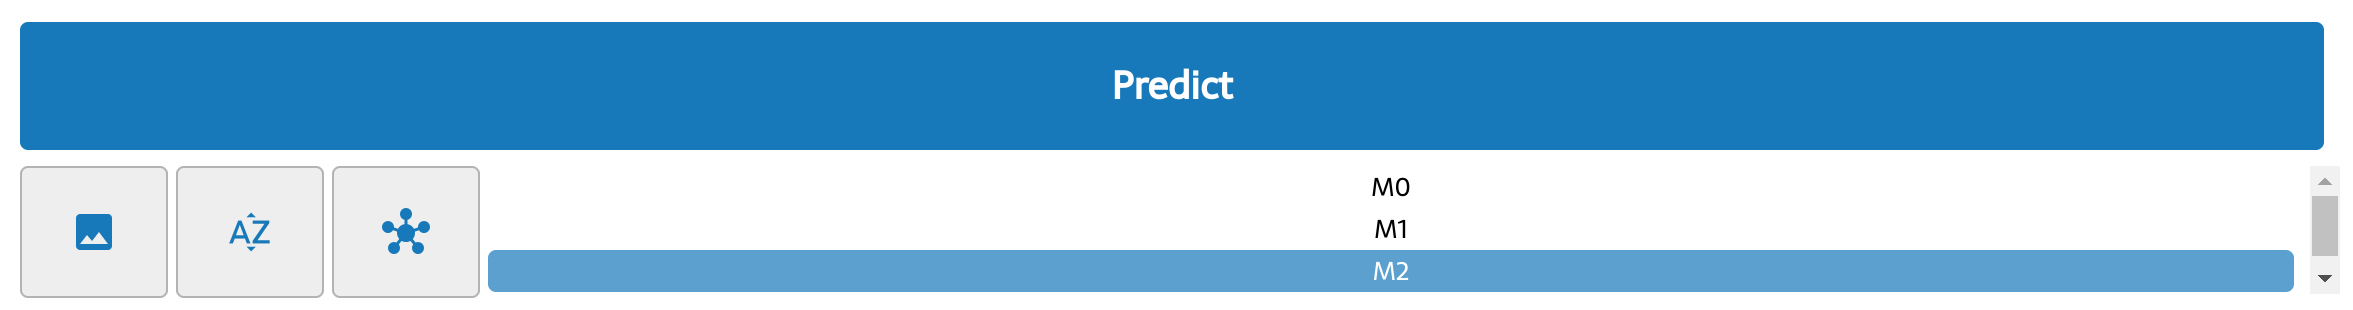
\includegraphics[width=0.9\textwidth]{imatges/results/selecting-model.png}
  \caption[Selecting exposed models by the API]{\textit{Selecting exposed models by the API. }}
  {\label{fig:selecting-model}}
\end{figure}

\end{enumerate}

Once we have loaded the images and selected the desired model for prediction,
we are ready to make the request to the API for inference using the chosen
model. The UI will display the images classified as melanoma with a red
background and the images classified as other classes with a blue background,
see Figure \ref{fig:after-prediction}. \\

On the top-right corner of every image appears button with a
square symbol. When you click on any of these buttons, a pop-up window appears,
providing additional information about the prediction for that specific image. \\

\begin{figure}[H]
  \centering
  \begin{adjustbox}{width=0.9\textwidth, trim={0cm 3.55cm 0cm 0cm}, clip}
    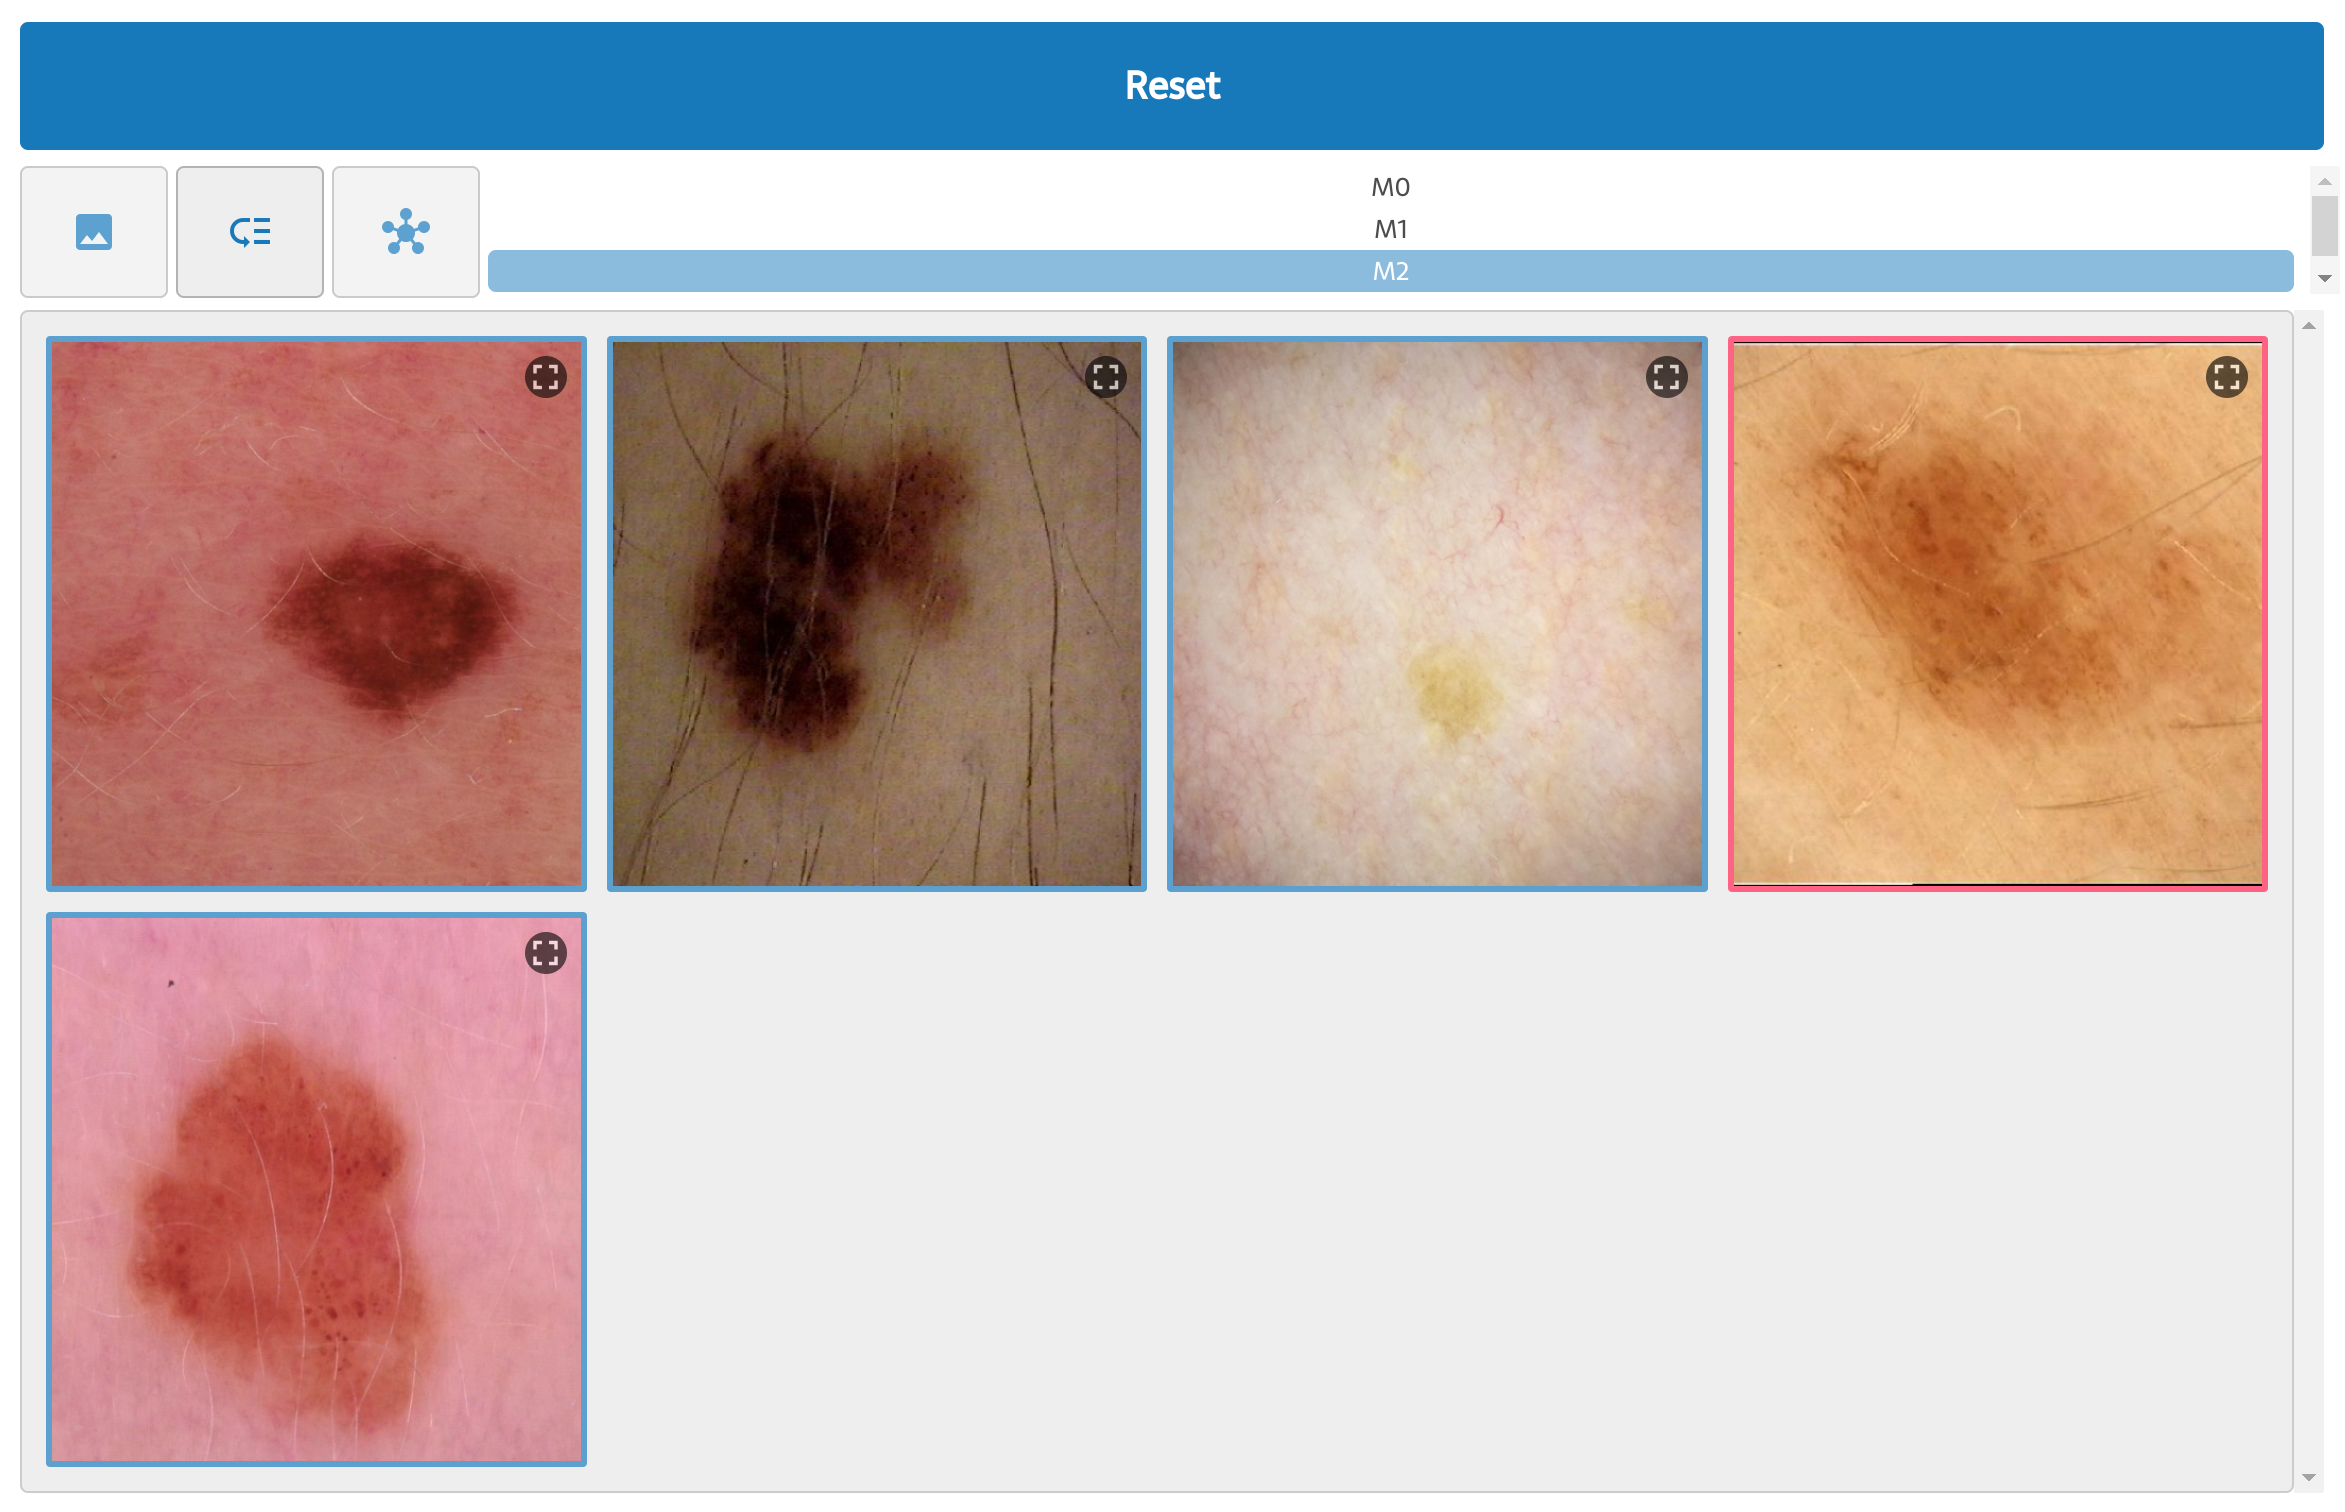
\includegraphics[width=\textwidth]{imatges/results/after-prediction.png}
  \end{adjustbox}
  \caption[UI state after prediction response]{\textit{UI state after prediction response.}}
  {\label{fig:after-prediction}}
\end{figure}


For instance, let's inquire about more information about the dermoscopy image
that was classified as melanoma in Figure \ref{fig:after-prediction}. Clicking
on the corresponding square button will trigger a pop-up as showed in Figure
\ref{fig:extra-inf-popup}. The pop-up provides extra information about the
prediction, image, mode's author, etc.

\begin{figure}[H]
  \centering
  \begin{adjustbox}{width=0.9\textwidth, trim={0.05cm 0cm 0.25cm 0cm}, clip}
    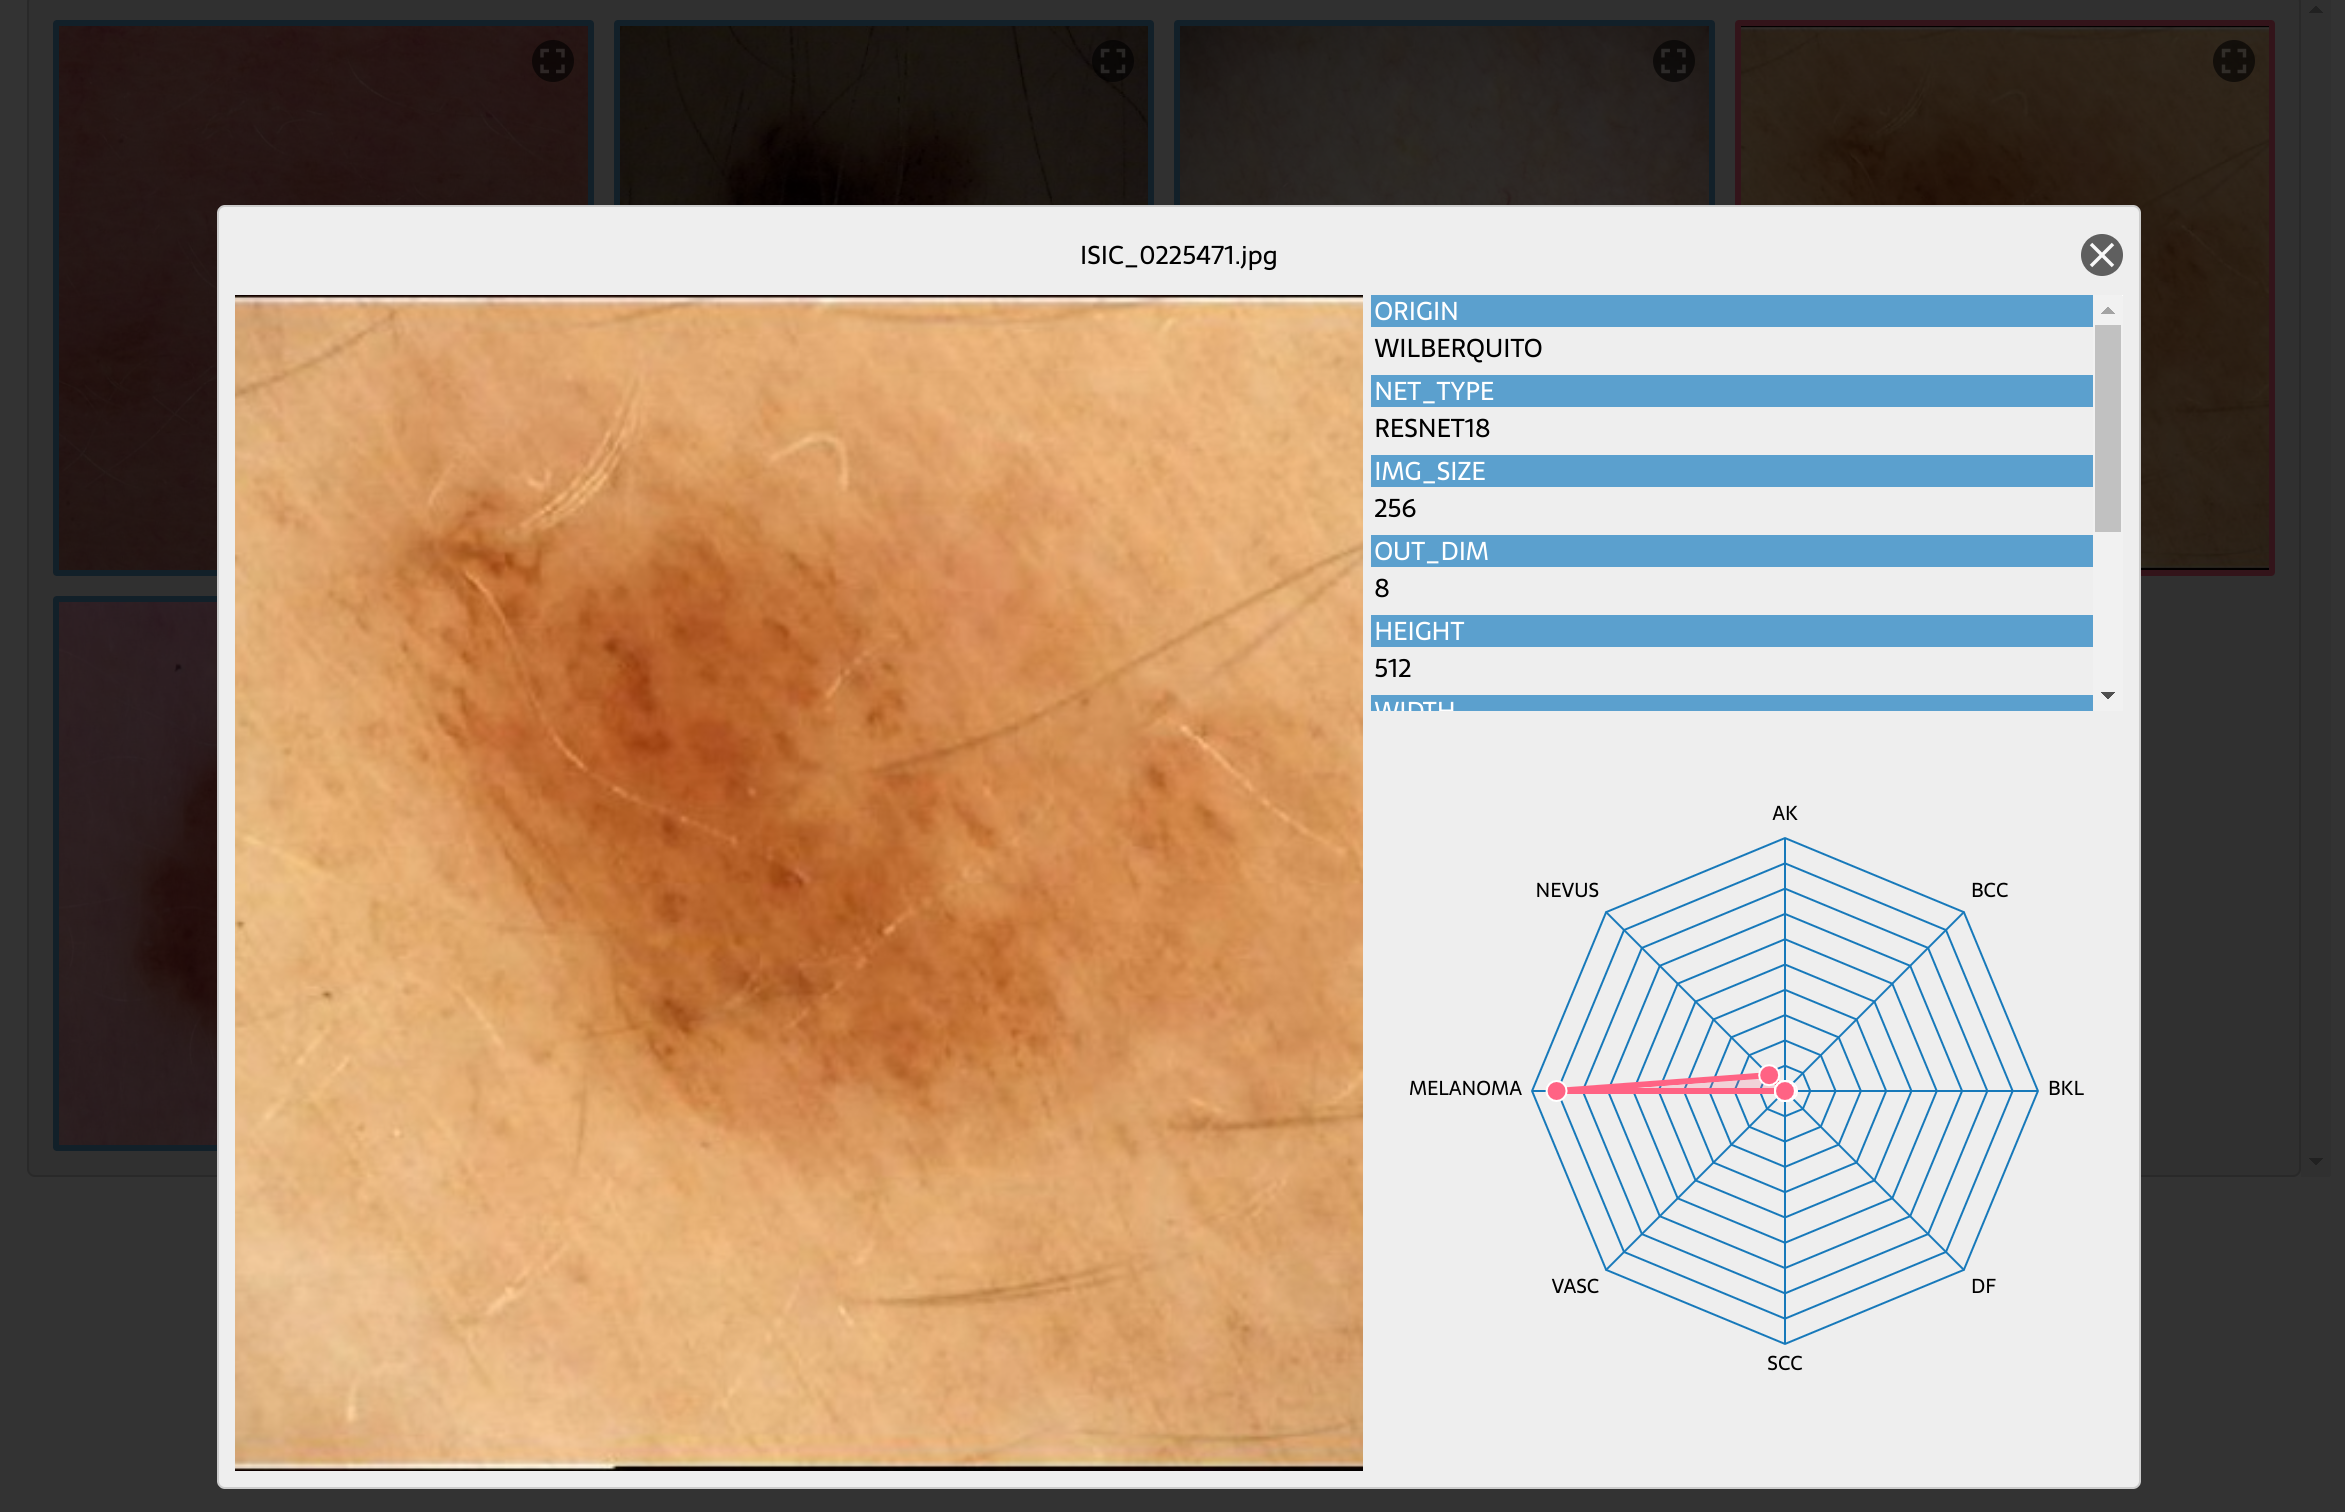
\includegraphics[]{imatges/results/extra-inf-popup.png}
  \end{adjustbox}
  \caption[Extra prediction information]{\textit{Extra prediction information.}}
  {\label{fig:extra-inf-popup}}
\end{figure}


\section{Conclusions and Future Work}
\label{cap:concl}

The main goal of this thesis was to utilize machine learning techniques to
train multiple CNNs models for detecting melanoma in an imbalanced dataset of
dermoscopy images, adding value creating a CAD infrastructure to make models easy
available to make predictions. \\

While the models were in the training phase, we took the opportunity to develop
the CAD (Computer-Aided Diagnosis) infrastructure. For the API, we opted for a
soft-configuration approach, where the configurations are specified through
file-based configurations, providing flexibility and ease of management.
Additionally, we designed a simple and intuitive user interface (UI) to
streamline the interaction of healthcare professionals with the exposed models.
\\

Furthermore, we achieved a significant milestone by successfully implementing a
mechanism for deploying the models and services using containers. By leveraging
containers, we ensured that the entire CAD architecture could be easily
replicated and deployed across different environments. To further simplify the
setup process, we also developed a shell script capable of downloading the
necessary images and initiating the container services effectively. \\

This approach combined both research and engineering efforts, enabling us to
make sophisticated knowledge accessible to a wider audience. By integrating
cutting-edge research and engineering principles, we have created a powerful
tool for medical professionals, providing them with advanced diagnostic
capabilities to improve patient care and outcomes. \\

As we assess the current state of the CAD infrastructure, we recognize the
existence of various potential implementations that could enhance its
capabilities. One promising approach involves establishing a mechanism for
iterative model training, continuously monitoring and tracking their
performance. Models exhibiting exceptional behavior could be promptly exposed
and made available for use. In the user interface (UI), professionals can
access the training results of the models, even in instances where the selected
model may not have performed optimally. By providing this additional
information, our goal is to boost professionals' confidence, preventing them
from relying blindly on the models' inferences. \\

Another promising approach involves exploring more complex Convolutional Neural
Network (CNN) models or other architectures, such as the Transformer
\cite{Transformer}. Finally, we could train our models with patient metadata
and expand the dataset. \\

{\bf The resulting CAD infrastructure is a tool to assist, not a replacement for
human expertise in desition making.}
